%% source: 2023-sp-redemption_midterm_01
%% tags: [time complexity]
\begin{prob}
    Suppose \mintinline{python}{bar} and \mintinline{python}{baz} are two functions.
    Suppose \mintinline{python}{bar}'s asymptotic time complexity is $\Theta(n^4)$, while
    \mintinline{python}{baz}'s is $\Theta(n)$.

    Suppose \mintinline{python}{foo} is defined as below:

    \begin{minted}{python}
        def foo(n):
            if n < 1_000_000:
                bar(n)
            else:
                baz(n)
    \end{minted}

    What is the asymptotic time complexity of \mintinline{python}{foo}?

    \begin{soln}
        $\Theta(n)$

        If you were to plot the function $T(n)$ that gives the time taken by
        \mintinline{python}{foo} as a function of $n$, you'd see something like the below:

        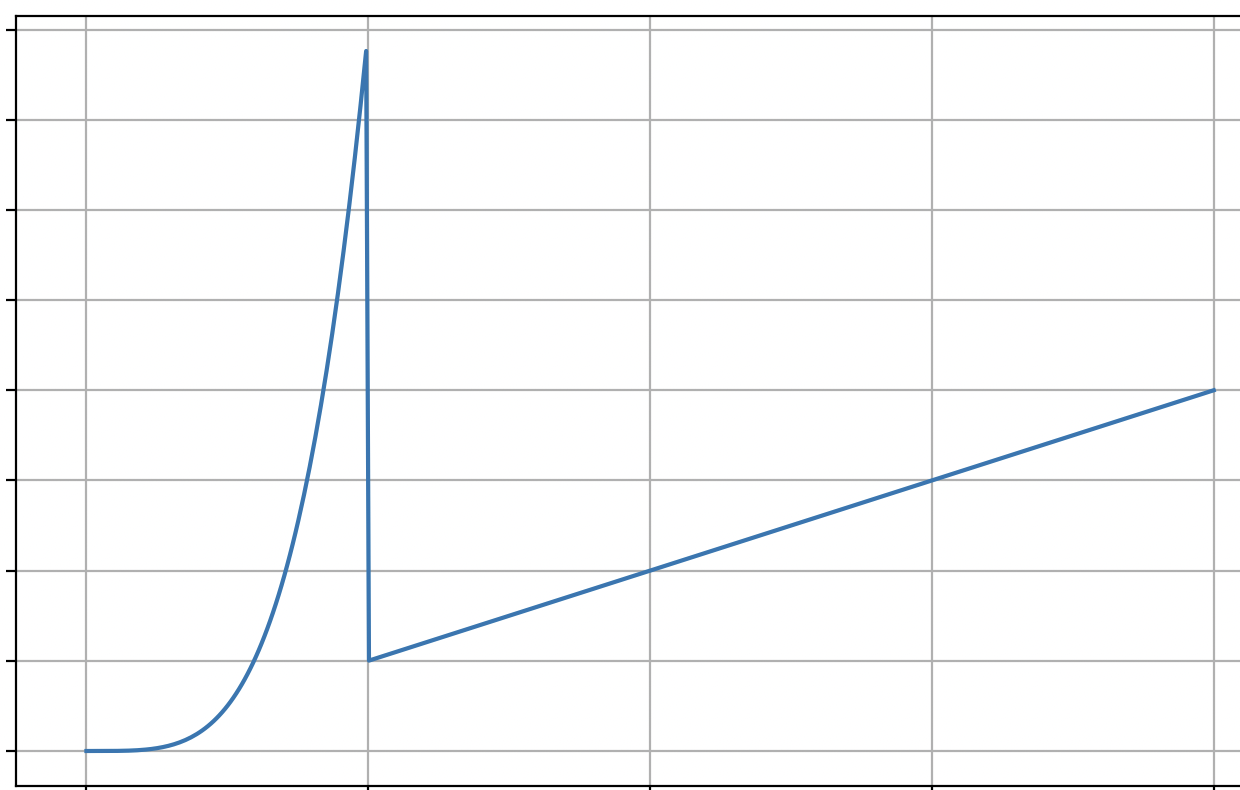
\includegraphics{./plot.png}

        This function starts off looking like $n^4$, but at $n = 1_000_000$, it
        "switches" to looking like $n$.

        Since asymptotic time complexity is concerned with the behavior of the
        function as $n$ gets large, we can ignore the part where $n$ is "small"
        (in this case, less than $1{,}000{,}000$). So, asymptotically, this function
        is $\Theta(n)$.

    \end{soln}
\end{prob}
